\documentclass[../SOP.tex]{standalone}

\usepackage{tikz}
\usetikzlibrary{calc}

\begin{document}


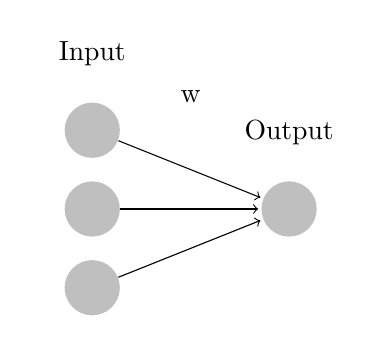
\begin{tikzpicture} [shorten >=1pt,->,draw=black,node distance=2cm, text height=2ex]
  \tikzstyle{every pin edge}=[<-, shorten <= 1pt]
  \tikzstyle{neuron}=[circle,fill=black!25,minimum size=17pt,inner sep=0pt, text width=18pt, text centered]
  \tikzstyle{annot} = [text width=4em, text centered,node distance=1cm]

  \foreach \name / \y in {1,...,3}
    \node[neuron] (I-\name) at (0,1-\y) {};
    \node[neuron] (O) at (2.5cm, -1) {};
  \foreach \source in {1,...,3}
    \path (I-\source) edge (O);

  \node[annot, above of=I-1] (ti) {Input};
  \node[annot, above of=I-1] (w) at ($(I-1)!0.5!(O)$) {w};
  \node[annot, above of=O] (to) {Output};

\end{tikzpicture}

\end{document}
